O condensador é a próxima etapa após o gás sair do compressor com uma alta temperatura e pressão. Ele é responsável pela troca de calor entre o fluido refrigerante e o meio, já que o ar, mais frio, passará pelos tubos do condensador, mais quente, e assim o fluxo de calor passará do fluido para o meio por meio do processo de convecção\cite{embracocolecao}.

Para a escolha do condensador, analisou-se o sistema de refrigeração como um todo. O ar frio que sairia do evaporador faria a troca de calor com o condensador, desse modo, não haveria a necessidade de ter um condensador de ar forçado, ou seja, um condensador que usa ventiladores para forçar a passagem de ar por entre os tubos. 

Definido o condensador a ser utilizado no processo, a principal característica que deverá ser levada em conta para se escolher o modelo é a vazão necessária de ar, já que estamos nos referindo a um condensador simples que necessita de uma vazão de ar externa. 

O fornecedor que melhor atende as restrições do sistema é a ElginTM. Assim, analisando seus modelos de condensadores, foi escolhido o modelo CDE-2812. Essa escolha é justificada pela vazão necessária nesse modelo que se assemelha numericamente, aproximadamente 75\%, com a vazão do evaporador escolhido. 

A imagem abaixo apresenta os dados técnicos do condensador escolhido.
\begin{figure}[!htbp]
	 \centering
	  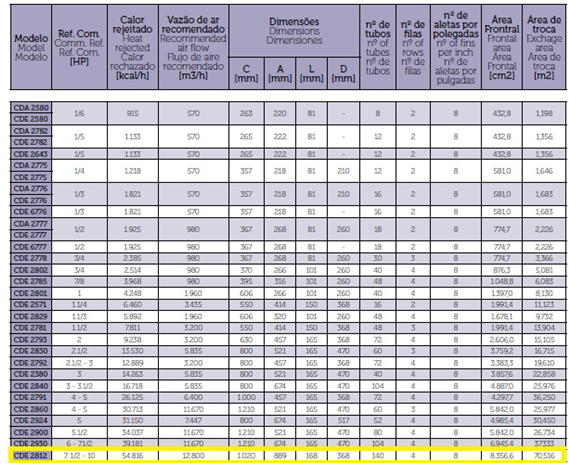
\includegraphics[scale=1]{editaveis/figuras/dados_tecnicos}
	  \caption[Dados técnicos do condensador]{Dados técnicos do condensador CDE-2812 em destaque no quadro amarelo\footnotemark}
	  \label{condensador}
	\end{figure}	   
	\footnotetext{Disponível em: https://www.elgin.com.br/portalelginadm/Upload/Downloads/refrigeracao/Folhetos\%20-\%2011-06-12/Condensadores.pdf}
	\FloatBarrier
	
\begin{figure}[!htbp]
	 \centering
	  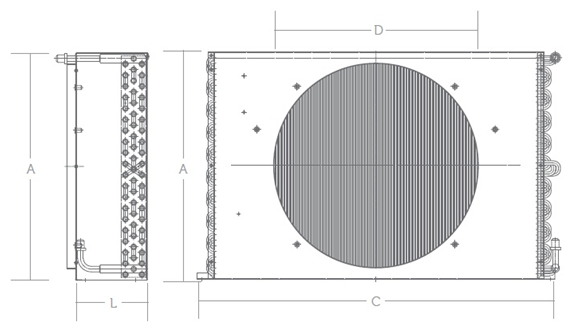
\includegraphics[scale=1]{editaveis/figuras/cotas_condensador}
	  \caption[Cotas do condensador]{Cotas do condensador\footnotemark}
	  \label{condensador}
	\end{figure}	   
	\footnotetext{Disponível em: https://www.elgin.com.br/portalelginadm/Upload/Downloads/refrigeracao/Folhetos\%20-\%2011-06-12/Condensadores.pdf}
	\FloatBarrier
	
\begin{figure}[!htbp]
	 \centering
	  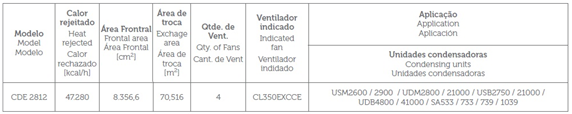
\includegraphics[scale=1]{editaveis/figuras/carac_tecnicas_condensador}
	  \caption[Características técnicas do condensador]{Características técnicas do condensador CDE-2812 \footnotemark}
	  \label{condensador}
	\end{figure}	   
	\footnotetext{Disponível em: https://www.elgin.com.br/portalelginadm/Upload/Downloads/refrigeracao/Folhetos\%20-\%2011-06-12/Condensadores.pdf}
	\FloatBarrier
	
\begin{figure}[!htbp]
	 \centering
	  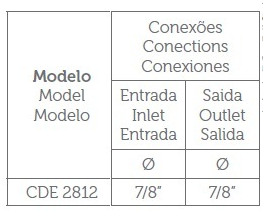
\includegraphics[scale=1]{editaveis/figuras/carac_tecnicas_conexao}
	  \caption[Características técnicas das conexões]{Características técnicas das conexões\footnotemark}
	  \label{condensador}
	\end{figure}	   
	\footnotetext{Disponível em: https://www.elgin.com.br/portalelginadm/Upload/Downloads/refrigeracao/Folhetos\%20-\%2011-06-12/Condensadores.pdf}
	\FloatBarrier


